\documentclass[tikz,border=5pt]{standalone}
\usepackage{amsmath}
\begin{document}
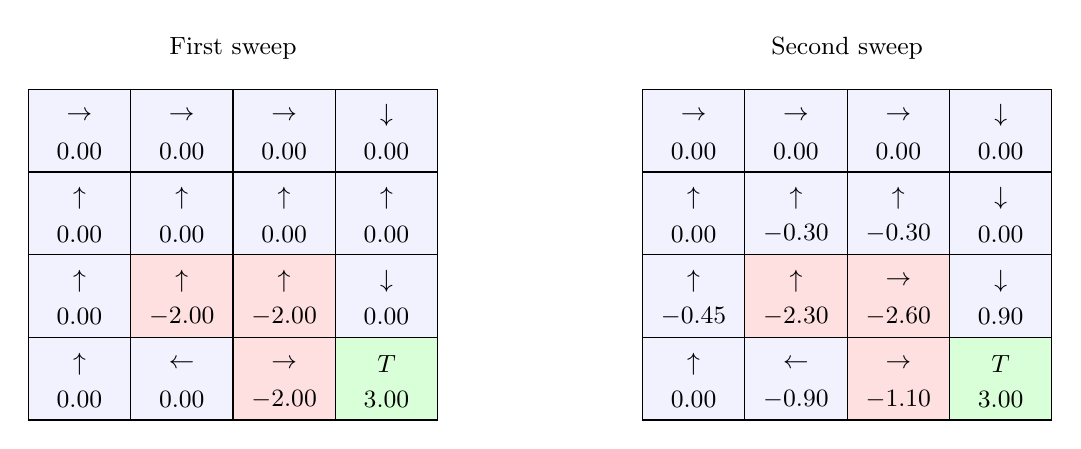
\begin{tikzpicture}[x=1.3cm,y=1.05cm,font=\small]
\node at (2,.5) {First sweep};
\fill[blue!5] (0,0) rectangle ++(1,-1);
\node at (0.5,-0.32) {$ \rightarrow $};\node at (0.5,-0.75) {$ 0.00 $};
\fill[blue!5] (1,0) rectangle ++(1,-1);
\node at (1.5,-0.32) {$ \rightarrow $};\node at (1.5,-0.75) {$ 0.00 $};
\fill[blue!5] (2,0) rectangle ++(1,-1);
\node at (2.5,-0.32) {$ \rightarrow $};\node at (2.5,-0.75) {$ 0.00 $};
\fill[blue!5] (3,0) rectangle ++(1,-1);
\node at (3.5,-0.32) {$ \downarrow $};\node at (3.5,-0.75) {$ 0.00 $};
\fill[blue!5] (0,-1) rectangle ++(1,-1);
\node at (0.5,-1.32) {$ \uparrow $};\node at (0.5,-1.75) {$ 0.00 $};
\fill[blue!5] (1,-1) rectangle ++(1,-1);
\node at (1.5,-1.32) {$ \uparrow $};\node at (1.5,-1.75) {$ 0.00 $};
\fill[blue!5] (2,-1) rectangle ++(1,-1);
\node at (2.5,-1.32) {$ \uparrow $};\node at (2.5,-1.75) {$ 0.00 $};
\fill[blue!5] (3,-1) rectangle ++(1,-1);
\node at (3.5,-1.32) {$ \uparrow $};\node at (3.5,-1.75) {$ 0.00 $};
\fill[blue!5] (0,-2) rectangle ++(1,-1);
\node at (0.5,-2.32) {$ \uparrow $};\node at (0.5,-2.75) {$ 0.00 $};
\fill[red!12] (1,-2) rectangle ++(1,-1);
\node at (1.5,-2.32) {$ \uparrow $};\node at (1.5,-2.75) {$ -2.00 $};
\fill[red!12] (2,-2) rectangle ++(1,-1);
\node at (2.5,-2.32) {$ \uparrow $};\node at (2.5,-2.75) {$ -2.00 $};
\fill[blue!5] (3,-2) rectangle ++(1,-1);
\node at (3.5,-2.32) {$ \downarrow $};\node at (3.5,-2.75) {$ 0.00 $};
\fill[blue!5] (0,-3) rectangle ++(1,-1);
\node at (0.5,-3.32) {$ \uparrow $};\node at (0.5,-3.75) {$ 0.00 $};
\fill[blue!5] (1,-3) rectangle ++(1,-1);
\node at (1.5,-3.32) {$ \leftarrow $};\node at (1.5,-3.75) {$ 0.00 $};
\fill[red!12] (2,-3) rectangle ++(1,-1);
\node at (2.5,-3.32) {$ \rightarrow $};\node at (2.5,-3.75) {$ -2.00 $};
\fill[green!15] (3,-3) rectangle ++(1,-1);
\node at (3.5,-3.32) {$ T $};\node at (3.5,-3.75) {$ 3.00 $};
\draw[step=1] (0,0) grid (4,-4);
\node at (8,.5) {Second sweep};
\fill[blue!5] (6,0) rectangle ++(1,-1);
\node at (6.5,-0.32) {$ \rightarrow $};\node at (6.5,-0.75) {$ 0.00 $};
\fill[blue!5] (7,0) rectangle ++(1,-1);
\node at (7.5,-0.32) {$ \rightarrow $};\node at (7.5,-0.75) {$ 0.00 $};
\fill[blue!5] (8,0) rectangle ++(1,-1);
\node at (8.5,-0.32) {$ \rightarrow $};\node at (8.5,-0.75) {$ 0.00 $};
\fill[blue!5] (9,0) rectangle ++(1,-1);
\node at (9.5,-0.32) {$ \downarrow $};\node at (9.5,-0.75) {$ 0.00 $};
\fill[blue!5] (6,-1) rectangle ++(1,-1);
\node at (6.5,-1.32) {$ \uparrow $};\node at (6.5,-1.75) {$ 0.00 $};
\fill[blue!5] (7,-1) rectangle ++(1,-1);
\node at (7.5,-1.32) {$ \uparrow $};\node at (7.5,-1.75) {$ -0.30 $};
\fill[blue!5] (8,-1) rectangle ++(1,-1);
\node at (8.5,-1.32) {$ \uparrow $};\node at (8.5,-1.75) {$ -0.30 $};
\fill[blue!5] (9,-1) rectangle ++(1,-1);
\node at (9.5,-1.32) {$ \downarrow $};\node at (9.5,-1.75) {$ 0.00 $};
\fill[blue!5] (6,-2) rectangle ++(1,-1);
\node at (6.5,-2.32) {$ \uparrow $};\node at (6.5,-2.75) {$ -0.45 $};
\fill[red!12] (7,-2) rectangle ++(1,-1);
\node at (7.5,-2.32) {$ \uparrow $};\node at (7.5,-2.75) {$ -2.30 $};
\fill[red!12] (8,-2) rectangle ++(1,-1);
\node at (8.5,-2.32) {$ \rightarrow $};\node at (8.5,-2.75) {$ -2.60 $};
\fill[blue!5] (9,-2) rectangle ++(1,-1);
\node at (9.5,-2.32) {$ \downarrow $};\node at (9.5,-2.75) {$ 0.90 $};
\fill[blue!5] (6,-3) rectangle ++(1,-1);
\node at (6.5,-3.32) {$ \uparrow $};\node at (6.5,-3.75) {$ 0.00 $};
\fill[blue!5] (7,-3) rectangle ++(1,-1);
\node at (7.5,-3.32) {$ \leftarrow $};\node at (7.5,-3.75) {$ -0.90 $};
\fill[red!12] (8,-3) rectangle ++(1,-1);
\node at (8.5,-3.32) {$ \rightarrow $};\node at (8.5,-3.75) {$ -1.10 $};
\fill[green!15] (9,-3) rectangle ++(1,-1);
\node at (9.5,-3.32) {$ T $};\node at (9.5,-3.75) {$ 3.00 $};
\draw[step=1] (6,0) grid (10,-4);
\end{tikzpicture}\end{document}